\documentclass{article}
\usepackage[margin=1in]{geometry}
\usepackage{pgfplots}
\usepackage{graphicx}
\pgfplotsset{compat=1.17}
\usepackage{tikz}
\usetikzlibrary{pgfplots.fillbetween} % for filling between paths

\begin{document}
\begin{figure}
  \centering
  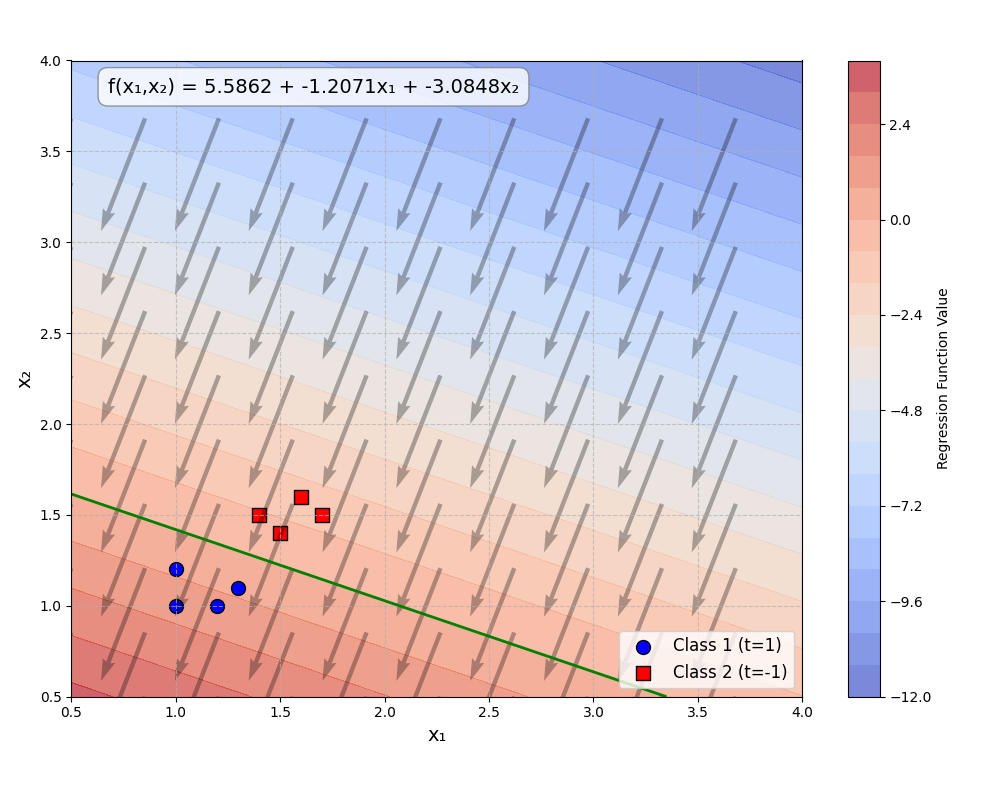
\includegraphics[width=0.4\textwidth]{Fig_1-1.png}
  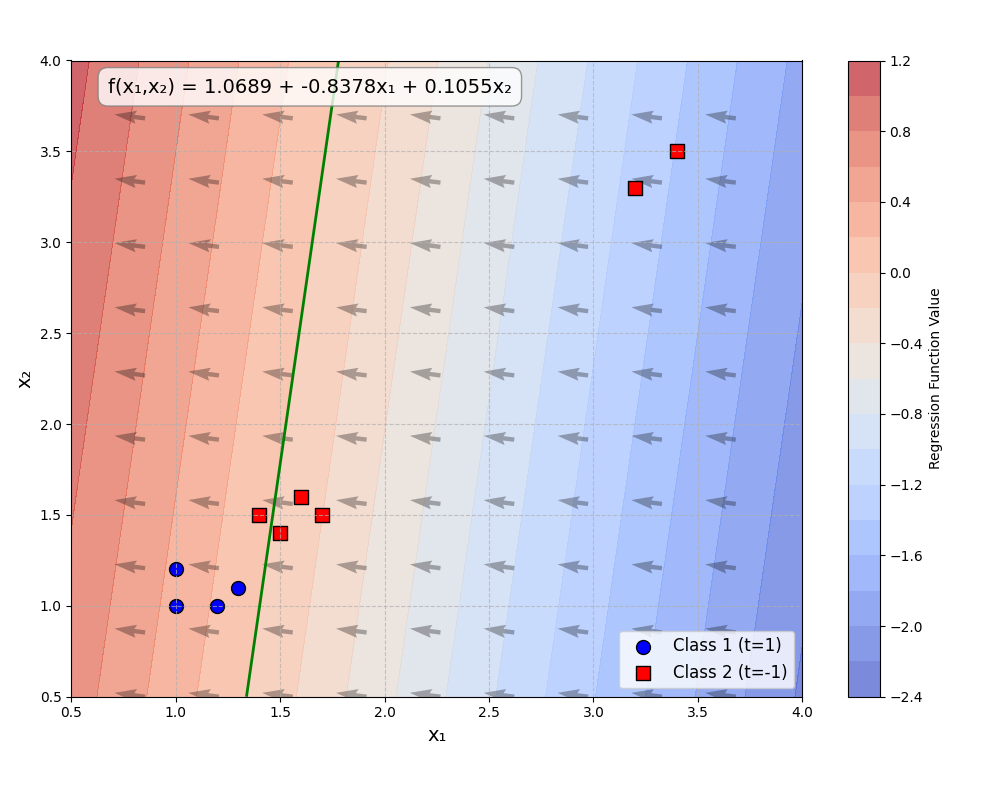
\includegraphics[width=0.4\textwidth]{Fig_1-2.png}
\end{figure}

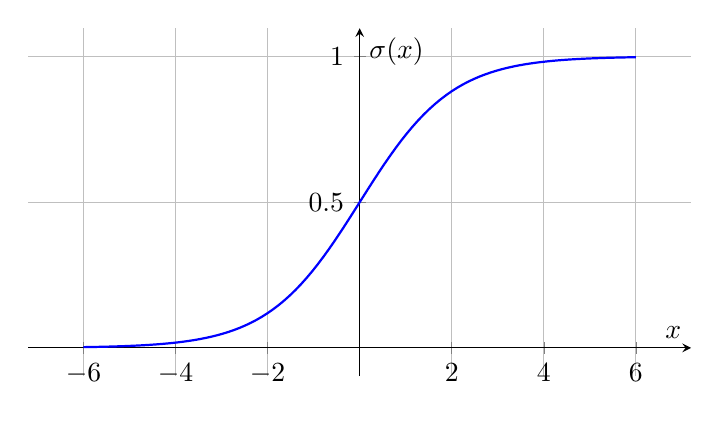
\begin{tikzpicture}
    \begin{axis}[
        axis lines = middle,
        xlabel = $x$,
        ylabel = {$\sigma(x)$},
        enlargelimits,
        xtick={-6,-4,...,6},
        ytick={0,0.5,1},
        domain=-6:6,
        samples=100,
        grid=both,
        width=10cm,
        height=6cm,
    ]
    \addplot[blue, thick] {1/(1+exp(-x))};
    \end{axis}
\end{tikzpicture}
\end{document}
